\chapter{Projektbeskrivelse}

\section{Projektgennemførelse}\label{Projektgennemfoerlse}
Projektet startede med, at der blev lavet en tidsplan, som var mulig at ændre undervejs, dog med faste deadlines, som skulle overholdes. De forskellige deadlines lagde op til, at der kunne arbejdes efter udviklingsmodeller, som er beskrevet nærmere i metodeafsnittet \ref{Metode}.\\ 
\\
Tidsplanen blev sidenhen ført mere detaljeret ind i projektstryringsværktøjet Scrum. Scrum blev benyttet til at holde overblikket over manglende, igangværende og afsluttede opgaver. Ligeledes blev værktøjet brugt som en kontakt mellem hardware-gruppen og software-gruppen, så begge grupper kunne holde sig opdateret på hinandens opgaver. For at prioritere arbejdsopgaverne er der blevet benyttet sprints af en uges varighed. Hver arbejdsopgave er blevet prioriteret med et antal points alt efter, hvor tidskrævende opgaven var, hvilket har været bestemmende for, hvor mange opgaver, der var mulighed for at lave i hvert sprint.\\
Gruppens seks medlemmer blev fra start delt op i to undergrupper, en med hovedfokus på hardware-udvikling, og en med hovedfokus på software-udvikling. Dog blev de basale dele til projektet, som kravspecifikation og scenarie udvalgt samlet. Scrum er her også et godt værktøj til at bevare overblikket over de to gruppers individuelle opgaver.\\ 
\\
Fra start blev der aftalt et ugentlig møde med vejleder og de to grupper som medvirkende parter. På denne måde blev alle parter holdt opdateret på udviklingsprocessen, især grupperne imellem, men også vejleder. Sidst i forløbet, under test af diverse dele af systemet, blev grupperne samlet og testene blev udarbejdet i fællesskab.\\ 
\\
Projektet er gennemført ved udarbejdelse af en samarbejdsaftale, herunder udvælgelse af en projektleder, som i tilfælde af uoverensstemmelse havde den afgørende stemme. 

\section{Metode} \label{Metode}
I metodeafsnittet beskrives, hvilke metoder og modeller, der er blevet brugt til gennemførsel og udvikling af projektet.\\
Der er desuden brugt versionsstyring igennem hele projektet til at holde styr på rettelser og versioner af dokumenter.\\ 
\subsection{ASE-modellen}
Den primære udviklingsmodel, der er benyttet i dette projekt, er ASE-modellen. ASE-modellen er en udviklingsmodel, der tager udgangspunkt i use cases. 
\begin{figure}[H]
	\centering
	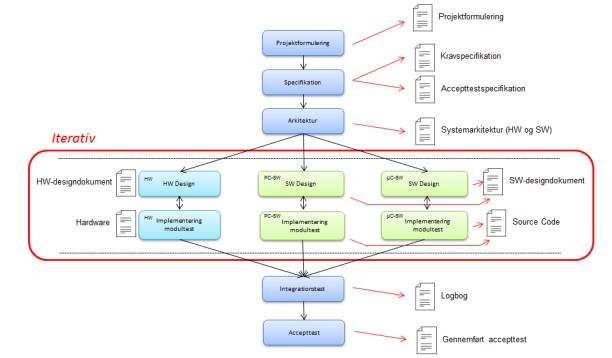
\includegraphics[width=1\textwidth]{Figurer/Metode/ASEmodellen}
	\caption{Projektmodel illustreret med de faser, som projektet gennemløber\protect\cite{IHA modellen}}
	\label{ASEmodel}
\end{figure}

Modellen er opbygget sådan, at udviklerne benytter vandfaldsmodellen (se afsnit \ref{Vandfald}) til at fastlægge en opgaveformulering, kravspecifikation og systemarkitektur, for derefter at designe og implementere de enkelte moduler i iterationer. \\ Ud fra projektformuleringen specificeres kravspecifikationen som en række use cases. En use case er et værktøj, der beskriver diverse aktørers interaktion med systemet. Ved at definere kravspecifikationen ud fra use cases, opnås et overblik over hvilke krav, der stilles til systemets endelige funktionalitet.\\ \\ Ud fra kravspecifikationen kan systemets accepttest udarbejdes. Efter kravspecifikationen er fastlagt, udarbejdes systemarkitekturen.\\ I systemarkitekturen opdeles systemets funktionalitet i moduler og deres grænseflader til resten af systemet bestemmes. Ud fra systemarkitekturen designes systemet ved at nedbryde det efter funktionalitet, som kan bindes til både hardware og software.
\subsection{Vandfald}\label{Vandfald}
Denne metode bygger på at gøre en hel fase af arbejdet færdigt, før den næste startes. Grafisk ser det ud som på figur \ref{Vandfaldsmodel}: \\

\begin{figure}[H]
	\centering
	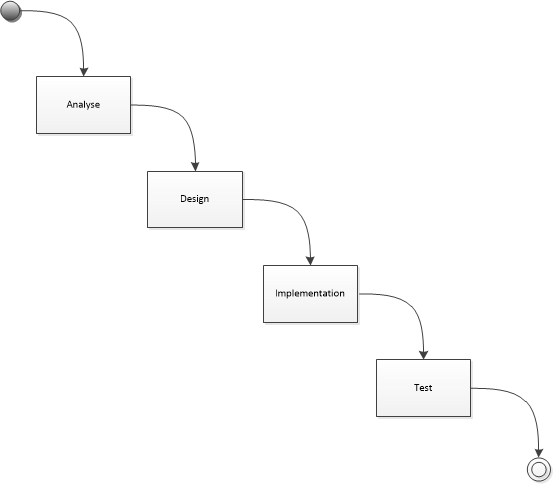
\includegraphics[width=0.8\textwidth]{Figurer/Metode/Vandfald}
	\caption{Vandfaldsmodel}
	\label{Vandfaldsmodel}
\end{figure}
Projektet starter med en analyse og videre til de andre faser - design, implementering og test. Det er altså hele systemet, der arbejdes igennem i hver fase, og vandfaldet symboliserer, at der kun arbejdes i en retning, altså kan man ikke gå imod strømmen. Metoden benyttes, når opgaven er veldefineret og velkendt. \\
Projekt forløbet skal have en kort varighed, dvs. mindre end ca. 4 måneder, under velkendte forhold med hensyn til udviklings- og testmiljø, udviklingsmetodik, platforme etc. \cite{Projektledelse}

\subsection{V-model}
V-modellen er en model, hvor testen planlægges parallelt med udviklingen. Accepttesten planlægges detaljeret efter kravnalysen, altså kravspecifikationen, systemtest planlægges detaljeret efter system design, og integrationstesten planlægges detaljeret efter arkitektur design fasen. Unit/modul testen ligger dog uændret i forhold til den traditionelle strategi.

\begin{figure}[H]
	\centering
	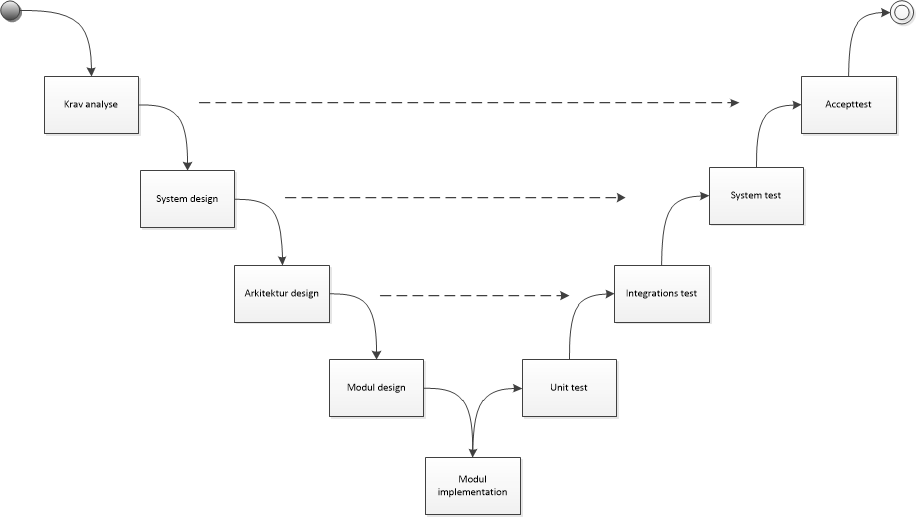
\includegraphics[width=1\textwidth]{Figurer/Metode/Vmodel}
	\caption{V-model}
	\label{Vmodel}
\end{figure}

Testens praktiske udførelse er altså uændret i forhold til ASE-modellen og vandfaldsmodellen, dvs. den ligger sidst i forløbet. Det betyder, at testfaserne planlægges modsat den rækkefølge, de udføres i. Den største forskel for testene er, at planlægningen baseres på de tidlige modeller af systemet og ikke på det færdige system. \\
 V-modellen udvides desuden med reviews og deadlines (se afsnit \ref{Projektgennemfoerlse}).

\subsection{SysML}
 I beskrivelsen af systemarkitekturen og det detaljerede design for det færdige produkt, er der anvendt SysML. SysML stammer oprindeligt fra UML, dog er UML hovedsagligt centreret omkring udvikling af software-systemer og er heraf også benyttet til det formål. Da det udviklede system både består af hardware og software, er der valgt både UML og SysML til beskrivelsen af arkitekturen.\\
Valget af SysML bunder også i, at det giver en god formidling af systemet - dette giver udviklerne et større overblik. Samtidig er det også let for en udenforstående at sætte sig ind i systemets kunnen.\\
I dette projekt er der benyttet struktur- og adfærdsdiagrammer til at specificere og dokumentere systemet. Som strukturdiagram er der anvendt et BDD og IBD.\\
Der er anvendt adfærdsdiagrammer i form af sekvensdiagrammer i dette projekt. Disse diagrammer er velegnet til sekventielt at beskrive den logiske funktionalitet i systemet. Softwaren er opbygget ud fra sekvensdiagrammer beskrevet i designafsnittet (se dokumentationen afsnit 3).

\section{Specifikation og analyse}
I udviklingen af hardwaren var der behov for, at mange af komponenterne blev nødt til at blive taget op til genovervejelse. \\
Der blev valgt at bruge en instrumentationsforstærker til forstærker-blokken i stedet for en operationsforstærker grundet instrumentationsforstærkerens reelle komponents tætte relation, til dens ideelle modpart. Da der blev arbejdet med meget små spændinger, var det vigtigt med en stor indgangsimpedans for at kunne forstærke disse små spændinger. Andre fordele ved instrumentationsforstærkeren indebærer let justerbar gain, samt høj common mode rejection ratio. \\
Dynamikområdet ved forstærkeren, blev oprindeligt fastlagt til at være højere end det endelige fastlagte dynamikområde. Dette blev justeret, fordi strømforsyningen og det oprindelige dynamikområde lå for tæt på hinanden. Det endelige dynamikområde blev valgt ud fra dynamikområderne til rådighed i DAQ'en. \\
Filterets overordnede design og komponenter var givet fra de krav, der var blevet sat til hardwaren fra starten af, og der var derfor ikke meget plads til ændringer af designet. Som spændingskilde blev Analog Discovery valgt, i stedet for et batteri, da Analog Discovery giver en stabil spænding, som ikke har behov for at blive afbalanceret. \\

Overvejelserne omkring designet af softwaren inden opstart på implementeringen var, at systemet skulle opfylde de opstillede krav i kravspecifikationen samt have en god brugergrænseflade.\\
Det blev hurtigt klart, at hvis software-systemet skulle fungere som ønsket, ville det blive nødvendigt at implementere systemet vha. tråde. Dette var nødvendigt, da der løbende var flere funktioner, der kørte samtidig. På den måde ville det være en god måde at forøge udnyttelsesgraden af systemet.\\
Tankerne om designet af brugergrænsefalden var at tage udgangspunkt i de 16 principper for gode brugergrænseflader.\cite{Usability} Ud fra disse principper blev designet af brugergrænsefladen udfærdiget til at være enkelt og brugervenligt for brugeren. Herudover gik designet på at få brugergrænsefladen til at se så virkelighedsnær ud som muligt. Derfor blev der lavet research af blodtryks-monitorer, hvorefter systemets brugergrænseflade er designet ud fra disse oplysninger. 

\chapter{Design, implementering og test}
   
\section{Hardware-design}
I dette afsnit beskrives udarbejdelsen af hardware-design og tilhørende tanker.

Der blev bestemt tideligt i forløbet at dele hardwaren op i to dele, en forstærkerdel og en filterdel. 
\\
\begin{figure}[H]
	\centering
	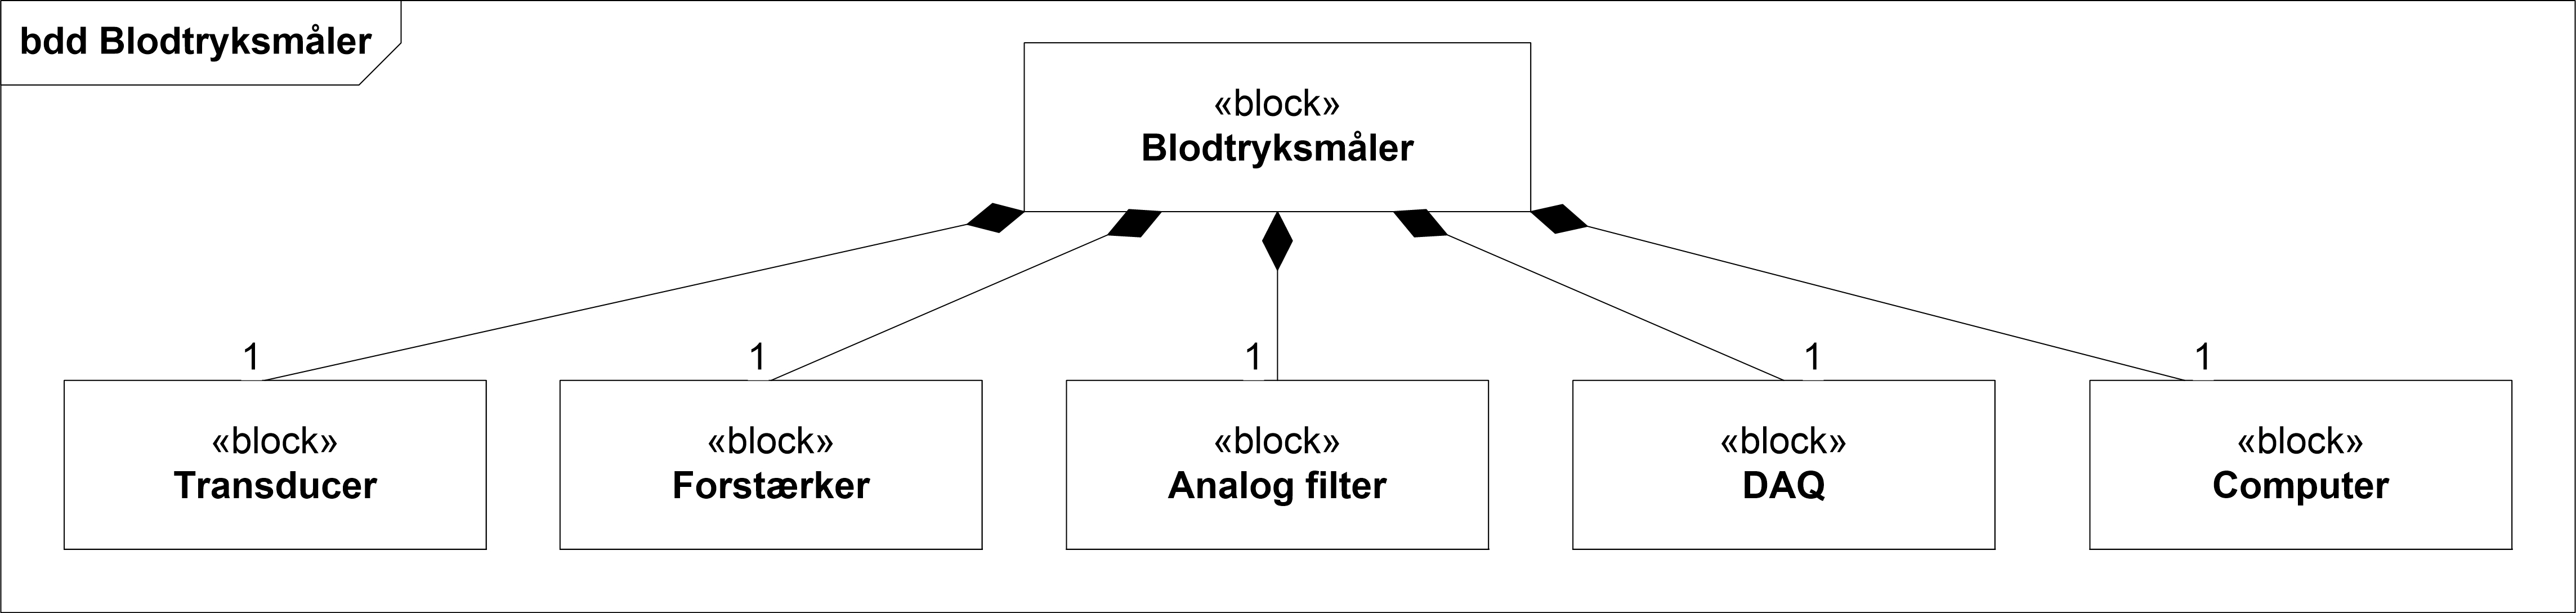
\includegraphics[width=1\textwidth]{Figurer/Hardware/BDD1}
	\caption{Blokdiagram for blodtryksmålingssystemet}
	\label{BDD blodtryksmaaler}
\end{figure}

Ud af blokdiagrammet, figur \ref{BDD blodtryksmaaler}, kan man se at blodtryksmålingssystemet består af fem dele. En transducer, som omformer tryk til spænding, en forstærker, et analogt 2.ordens lavpasfilter, en DAQ og en computer. \\

Det første, der blev designet til fulde, var forstærkeren. Forstærkeren blev designet med tanke på, at det er meget små spændinger, som bliver målt fra transduceren. En almindelig operationsforstærker blev derfor fravalgt, og en instrumentationsforstærker blev valgt i stedet. Vejleder anbefalede typen INA114, grundets denne types gode common mode rejection ratio og høje reelle indgangsimpedans. Kredsløbet blev som vist på figur \ref{forstkreds}. \\

\begin{figure}[H]
	\centering
	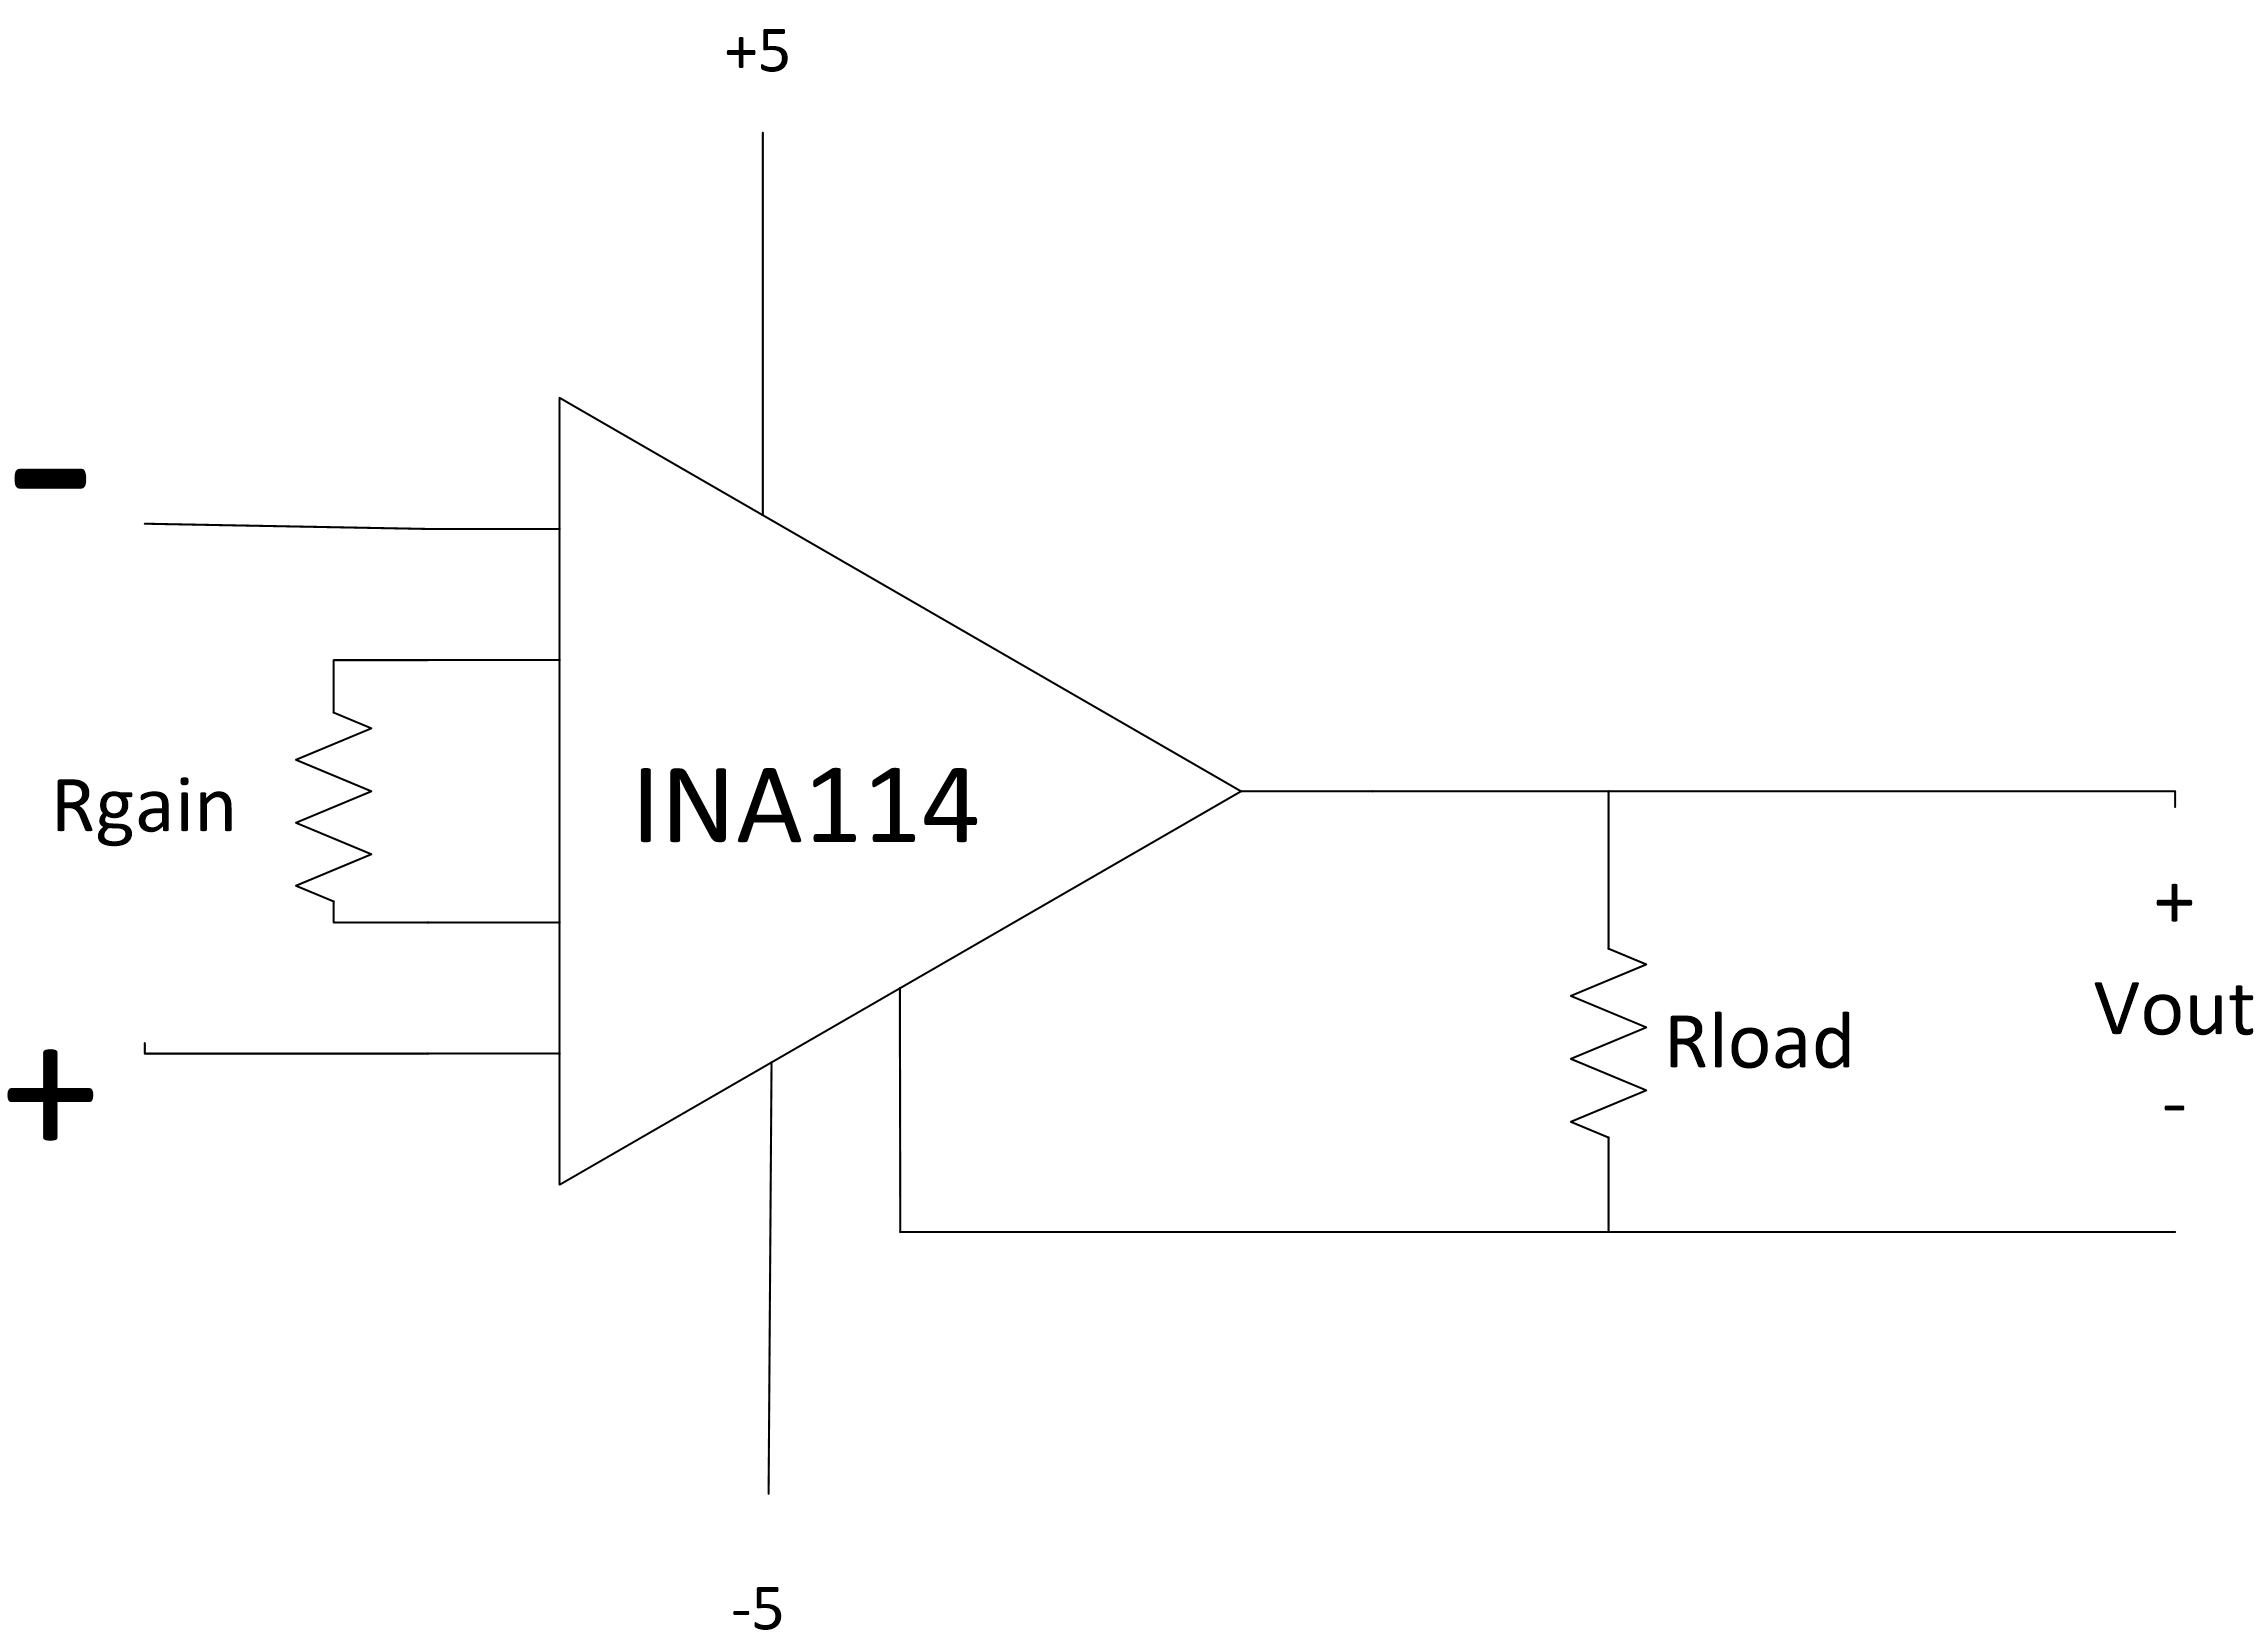
\includegraphics[width=0.6\textwidth]{Figurer/Hardware/Forstaerker}
	\caption{Der overordnede design af forstærkeren.}
	\label{forstkreds}
\end{figure}

Som set på figur \ref{forstkreds}, er R$_{gain}$ modstanden, som bestemmer forstærkningen, og R$_{load}$ repræsenterer den belastning, der kommer efter forstærkeren. 

Komponentværdier for forstærker er herefter udregnet. Disse udregninger kan ses i dokumentationen i afsnit 3.2.1, og komponentlisten for forstærkeren kan ses i afsnit \ref{himpl}. 

Det næste, der skulle designes, var filteret. Filteret skulle realiseres som et aktivt 2. ordens lavpasfilter af typen Sallen-Key med unity gain og med en båndbredde på 50Hz. Filteret blev yderligere specificeret til at skulle være et Butterworth-filter, med en cutoff-frekvens på 50Hz. Yderligere var visse komponentværdier forhåndsbestemt. Designet af filteret kan ses på figur \ref{fig:rFilter}.

\begin{figure}[H]
	\centering
	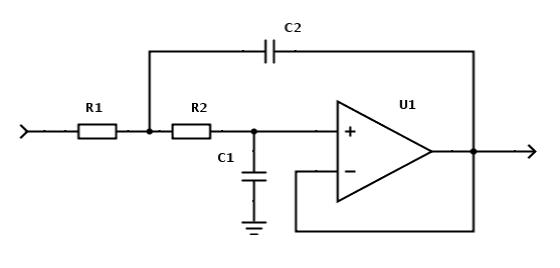
\includegraphics[width=1\textwidth]{Figurer/Hardware/FilterDesign}
	\caption{Unity gain 2. ordens Sallen-Key lavpas konfiguration}
	\label{fig:rFilter}
\end{figure}

Et Butterworth-filter har en anderledes $\zeta$ grundet anderledes prioriteter i forhold til frekvensområdet. Der blev brugt en hjemmeside til at finde overføringsfunktionen for det givne filter \cite{Overforing}. Herefter blev komponentværdierne teoretisk udregnet. Udregningerne kan ses i dokumentationen, afsnit 3.2.2. De endelige værdier for komponenterne, kan ses på komponentlisten for filteret i afsnit \ref{himpl}. 
   
   
\section{Software design}\label{Software arkitektur}
   I software designet er der udarbejdet en domænemodel, der giver et overblik over hele systemet.
   
 \begin{figure}[H]
	\centering
	\includegraphics[width=1\textwidth]{Figurer/ISE/Domaenemodel}
	\caption{Domænemodel}
	\label{domaenemodel}
\end{figure}

I domænemodellen er relationerne mellem aktørerne og systemets dele beskrevet med pile og vejledende tekster, hvilket gerne skulle give et større overblik over systemets funktionalitet. \\ 
En domænemodel beskriver dog ikke, hvilken rækkefølge de forskellige handlinger sker i, og derfor er der udarbejdet sekvensdiagrammer for hver use case for systemet, som skal beskrive dette.\\
Nedenfor på figur \ref{sekvensdiagram} ses sekvensdiagrammet for use casen "Mål blodtryk":

\begin{figure}[H]
	\centering
	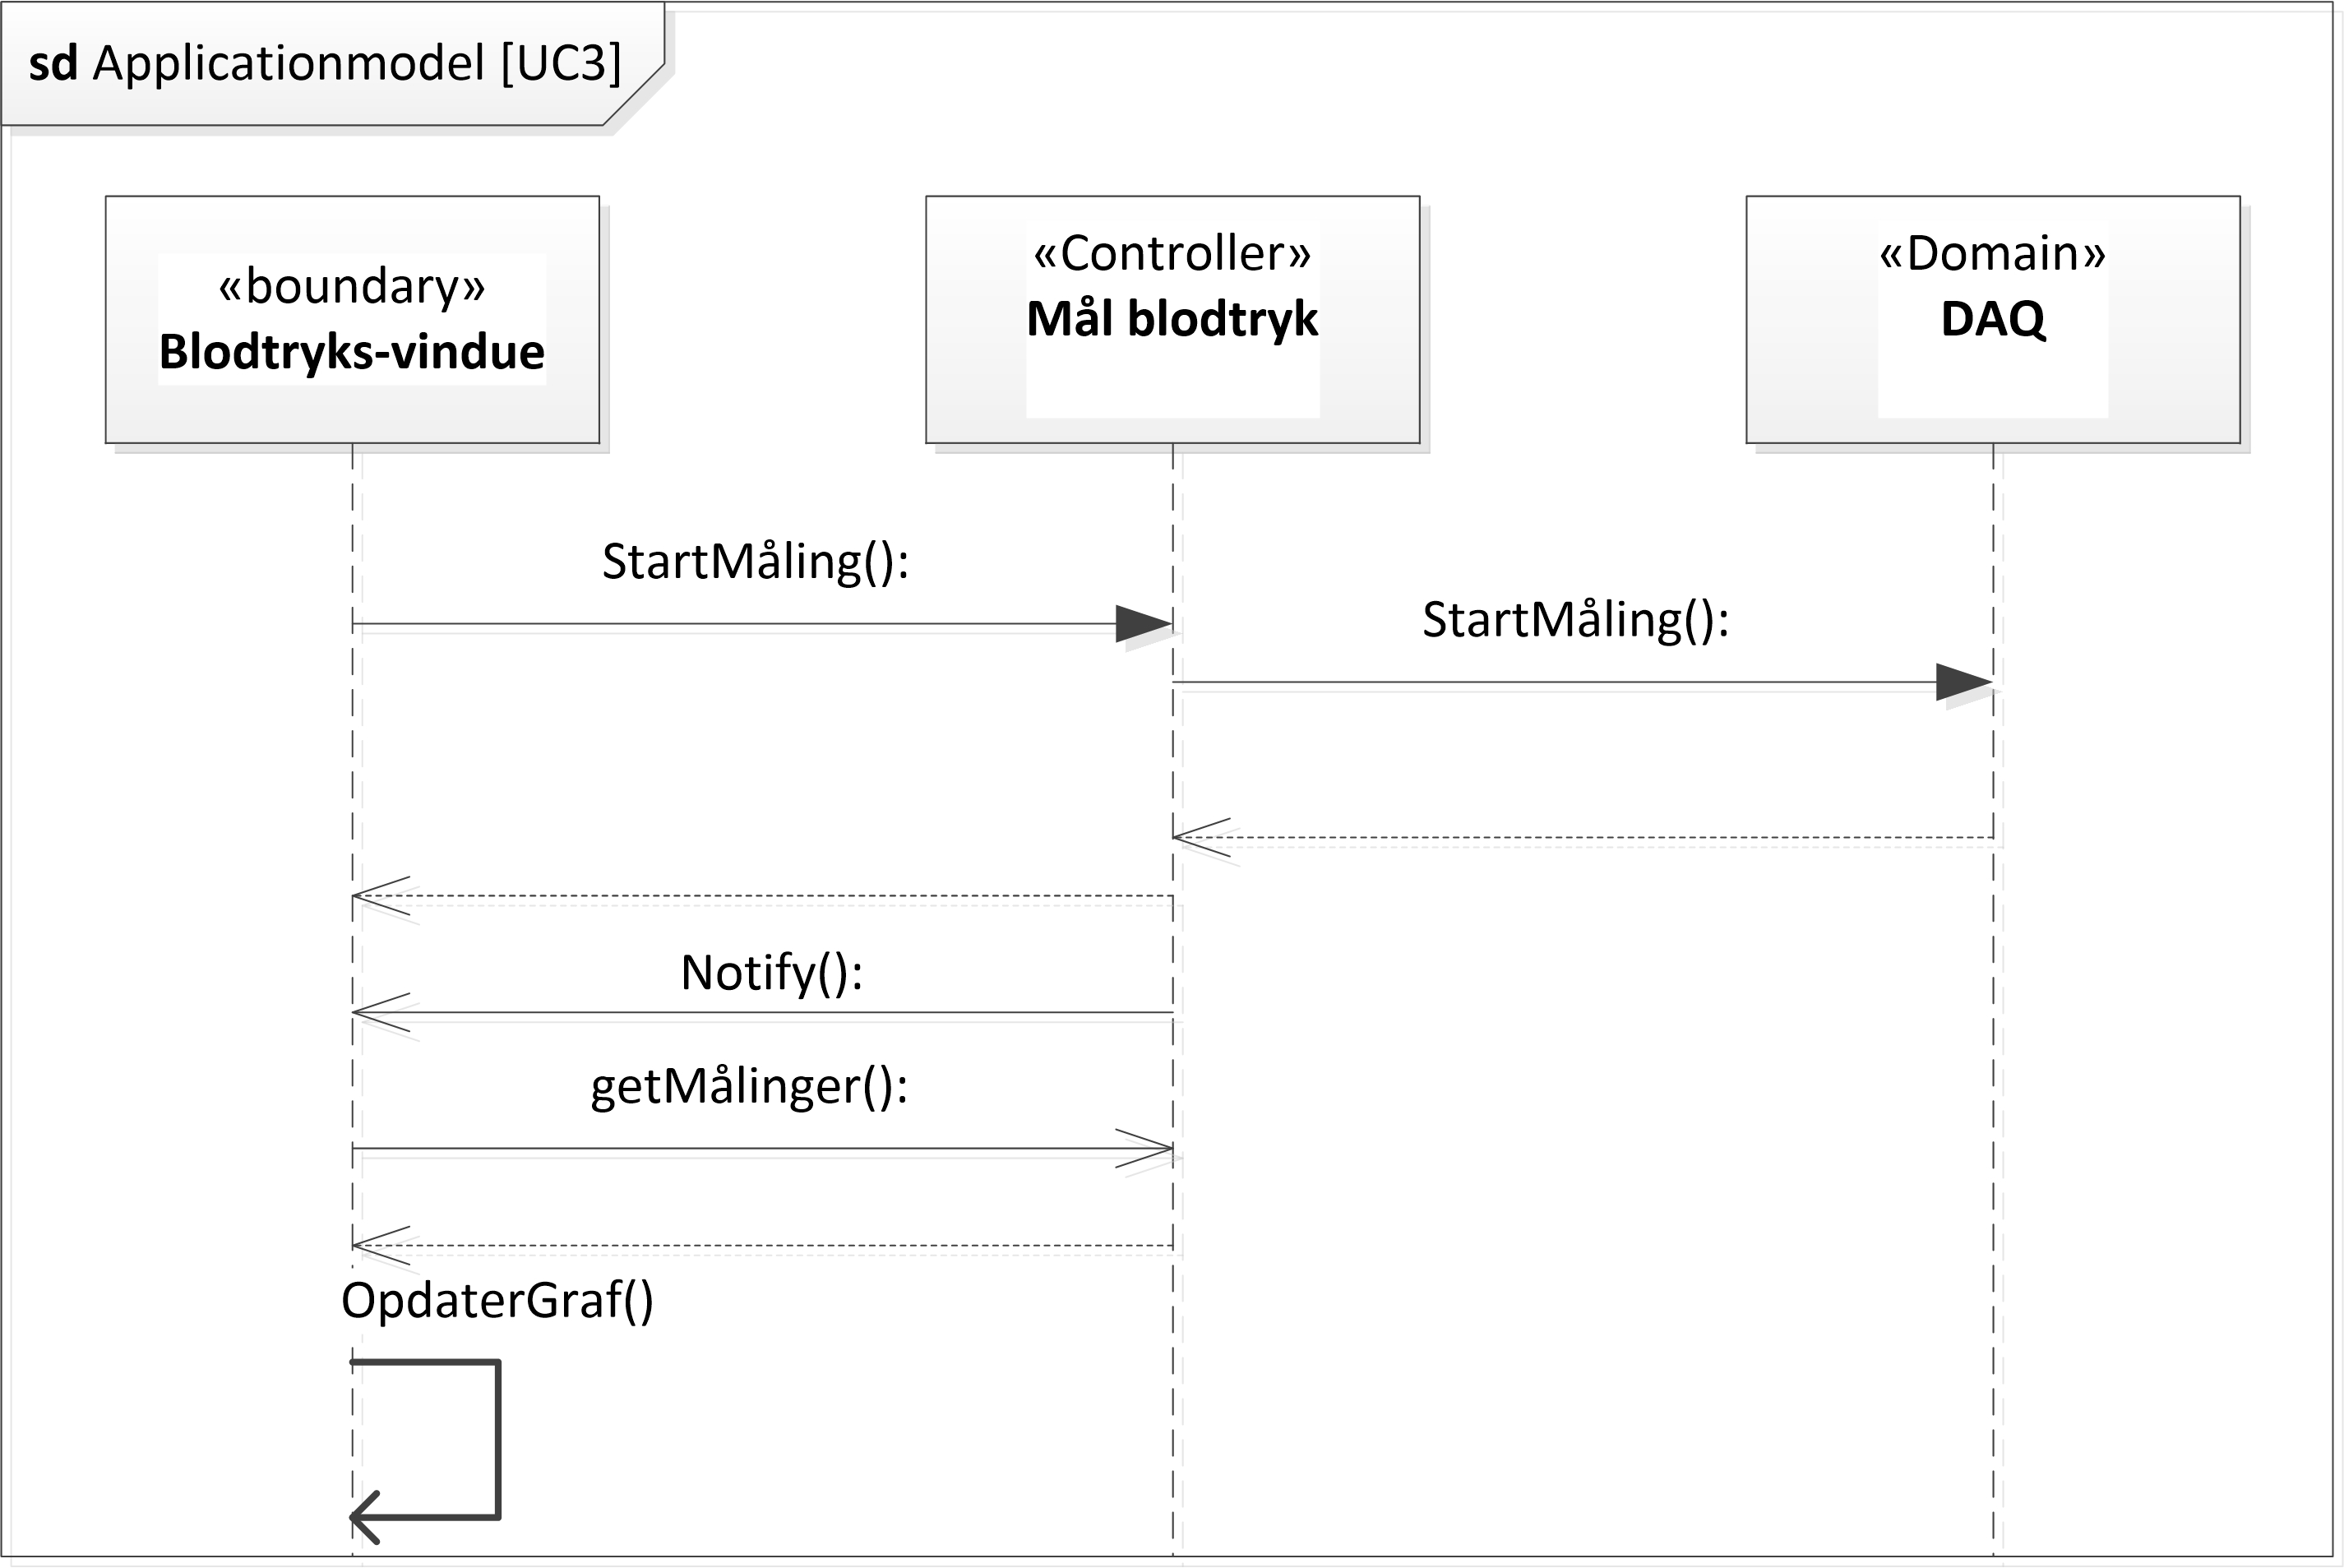
\includegraphics[width=1\textwidth]{Figurer/ISE/sdAppModelUC3}
	\caption{Sekvensdiagram UC3}
	\label{sekvensdiagram}
\end{figure}

Figur \ref{sekvensdiagram} viser, hvordan brugeren interagerer med brugergrænsefladen ved at starte blodtryksmålingen. Herefter bliver metoden til at starte blodtryksmålingen kaldt ned gennem logik- og datalag hvorefter målingen vises i en graf på brugergrænsefladen. Grafen bliver hele tiden opdateret med nye målinger.\\
Ud fra dette kan det ses, hvordan brugerens interaktion med brugergrænsefladen sætter gang i metoder i softwareprogrammet. Sekvensdiagrammet giver altså et overblik over, hvordan softwaren er bygget op.\\
Sekvensdiagrammerne for de øvrige use cases kan ses i dokumentationen afsnit 3.3.3.
  

\section{Hardware implementering}
\label{himpl}
Efter komponentudregningen, blev de to hardware-blokke bygget op. Det blev valgt at bygge forstærkeren og filteret seperat, grundet pladsmangel og sammenhæng. Opstillingen hertil ses på figur \ref{samletopbygning}.\\

\begin{figure}[H]
	\centering
	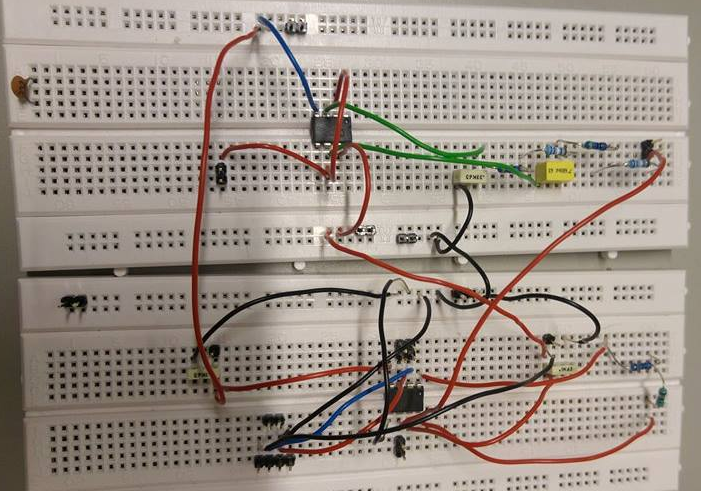
\includegraphics[width=1\textwidth]{Figurer/Hardware/samletopstilling}
	\caption{Opstilling af forstærker og filter}
	\label{samletopbygning}
\end{figure}

Grundet mangel på præcise modstande, blev modstandene delt op i to, både i filteret og forstærkeren, så det var muligt at komme så tæt på den ønskede modstandsværdi som muligt. \\
For forstærkeren blev styklisten som vist på tabel \ref{Forsttabel}.



\begin{table}[H]
\centering
\begin{tabular}{l l l l l}
\textbf{Komponent} & \textbf{Antal} & \textbf{Type}  &  &  \\ \cline{1-3}
Modstand           & 1              & 120$\Omega$   &  &  \\ \cline{1-3}
Modstand           & 1              & 4.8$\Omega$   &  &  \\ \cline{1-3}
Kondensator        & 2              & 100nF         &  &  \\ \cline{1-3}
Instrumentationsforstærker &    1   & INA114		     &  &  \\ \cline{1-3}
\end{tabular}
\caption{Forstærkertabel}
\label{Forsttabel}
\end{table}

Grundet forskel imellem teoretiske værdier og faktiske, er R$_{gain}$ 0,51$\Omega$ mindre end den skulle have været.\\
Den samlede stykliste for filteret blev som vist på tabel \ref{Filtertabel}.

\begin{table}[H]
\centering
\begin{tabular}{lllll}
\textbf{Komponent} & \textbf{Antal} & \textbf{Type}  &  &  \\ \cline{1-3}
Modstand           & 2              & 6.2k$\Omega$ &  &  \\ \cline{1-3}
Modstand           & 2              & 470$\Omega$   &  &  \\ \cline{1-3}
Kondensator        & 1              & 680nF         &  &  \\ \cline{1-3}
Kondensator        & 1              & 330nF         &  &  \\ \cline{1-3}
Operationsforstærker &    1         & OP27G          &  &  \\ \cline{1-3}
\end{tabular}
\caption{Filtertabel}
\label{Filtertabel}
\end{table}

I det analoge filter, er kondensatoren, C$_1$, i praksis 3,2nF mindre end  beregnet. Desuden er de to identiske modstande, R$_1$ og R$_2$, som i praksis er 17$\Omega$ mindre end teorien foreskriver.\\
Det blev vurderet, at afvigelserne var forholdsvidst små, og derfor er der valgt at se bort fra dem. For modstandene er der desuden 1 \% usikkerhed, hvilket betyder man alligevel ikke kan være helt sikker på komponentværdien.\\
En reel cutoff-frekvens blev herefter udregnet. Denne kan ses i ligning \ref{cutoff}.


\begin{align}
f_{c} = \frac{1}{2\pi \sqrt{R_{1}C_{1}R_{2}C_{2}}} = \frac{1}{2\pi \sqrt{6687 \cdot 333,2\times 10^{-9} \cdot 6687 \cdot 680\times 10^{-9}}} = 50,37 Hz
	\label{cutoff}
\end{align}
%\caption{Udregning af den reelle cutoff frekvens}

\section{Software implementering}
I software implementeringen er der beskrevet, hvordan systemet er blevet implementeret i form af teoretiske metoder og kodeudsnit, samt diagrammer over den implementerede kode.

\subsection{3-lagsmodellen}
Softwaren er implementeret ud fra 3-lagsmodellen. 3-lagsmodellen er bestående af lagene præsentationslag, logiklag og datalag. Denne opdeling af lagene gør det langt lettere at vedligeholde systemet, fordi der kan ændres i et enkelt lag, uden det har indflydelse på resten af programmet.\\ 
3-lagsmodellen er desuden en god software-arkitektur at bruge ved et system udarbejdet af en gruppe, da der kan arbejdes på to forskellige lag af to personer samtidigt, hvis bare grænsefladerne bliver overholdt.\\
Herudover er koden implementeret, så den har lav kobling og høj samhørighed således, at der har været mulighed for at teste kode elementer undervejs i processen. 

\subsection{Tråde}
Blodtrykmålingssystemet skal simultant opfange målinger og vise disse på brugergrænsefladen. Dette stiller nogle krav til softwareopbygningen, da kodestykker skal køre på samme tid. For at løse denne problemstilling, er der anvendt trådprogrammering. Trådprogrammering er et integreret værktøj i C\#, som giver mulighed for at køre flere ting samtidigt på flere kerner i computerens CPU.\\

\subsection{Observer}
Observermønstret er et mønster, hvor et objekt, kaldet et subject, informerer en liste af observers, når noget er ændret eller gennemført ved at kalde en af observerens metoder. Dette mønster har været nødvendigt at anvende, da grafen i brugergrænsefladen skal informeres om, hvornår der er nye data af hhv. logiklaget og datalaget. Det vil sige, at Logik-klassen og DAQ-klassen begge fungerer som subjects, mens GUI-laget og Logik-klassen fungerer som observers. Logik-klassen er subject for GUI, og Data-klassen er subject for Logik. Et eksempel på hvordan dette er bygget op ses i klassediagrammet på figur \ref{observerklasse}. Her kan man se, at Logik-klassen arver fra IObserver og ISubject, DAQklasse arver fra ISubject og Form1 arver fra IObserver.

\begin{figure}[H]
	\centering
	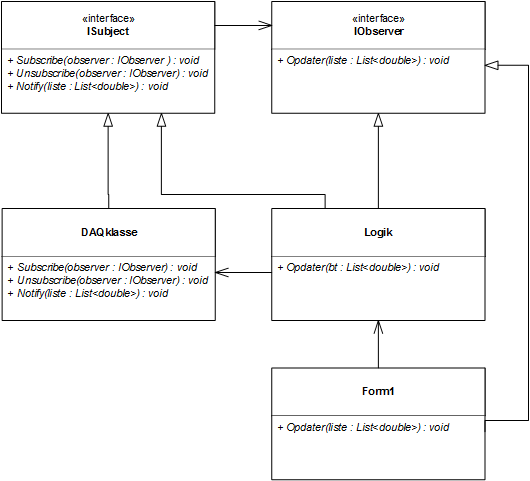
\includegraphics[width=1\textwidth]{Figurer/SoftwareImplementering/observer}
	\caption{Klassediagram over observermønsteret}
	\label{observerklasse}
\end{figure}

\newpage
\subsection{Kodeelementer \& diagrammer}
Nedenfor på figur \ref{kode3} og \ref{kode4} ses, hvordan metoden getGrafData() kører i sin egen tråd og sørger løbende for, at logiske operationer udføres på listen sideløbende med, at data hentes. Det er altså denne metode, der klargør listen til at blive vist på GUI’en. Det er også her, kalibreringsfaktoren ganges og offsettet trækkes fra på samtlige tal i listen.\\ 
Det bemærkes desuden, at de 20 målinger, der modtages fra DAQ-klassen er skåret ned til en ved at tage gennemsnittet af de tyve. På denne måde overbelastes systemet ikke ved at skulle vise 1000 målinger pr. sekund i en graf, men samtidig er alle målinger repræsenteret ligevægtigt.
\begin{figure}[H]
	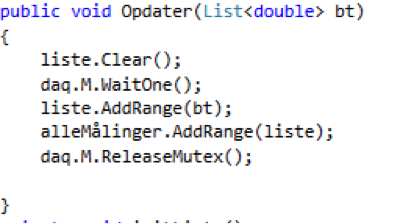
\includegraphics[width=0.6\textwidth]{Figurer/Jeppe/5}
	\caption{Metoden Opdater() som ligger i laget "Logik"}
	\label{kode3}
\end{figure}

\begin{figure}[H]
	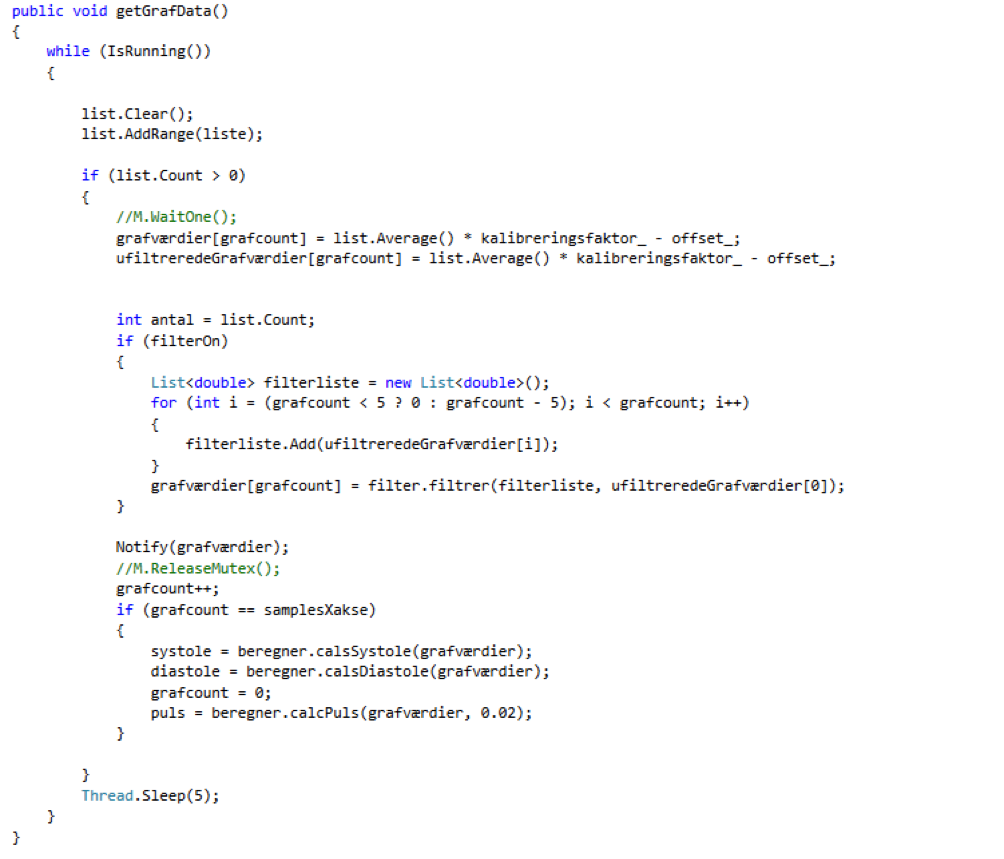
\includegraphics[width=1.3\textwidth]{Figurer/Jeppe/6}
	\caption{getGrafData() i laget Logik}
	\label{kode4}
\end{figure}

Nedenfor på figur \ref{UC3sekvens} ses et sekvensdiagram over use case 3, som viser sammenspillet mellem Form1, Logik og DAQklasse, når der foretages en måling:

\begin{figure}[H]
	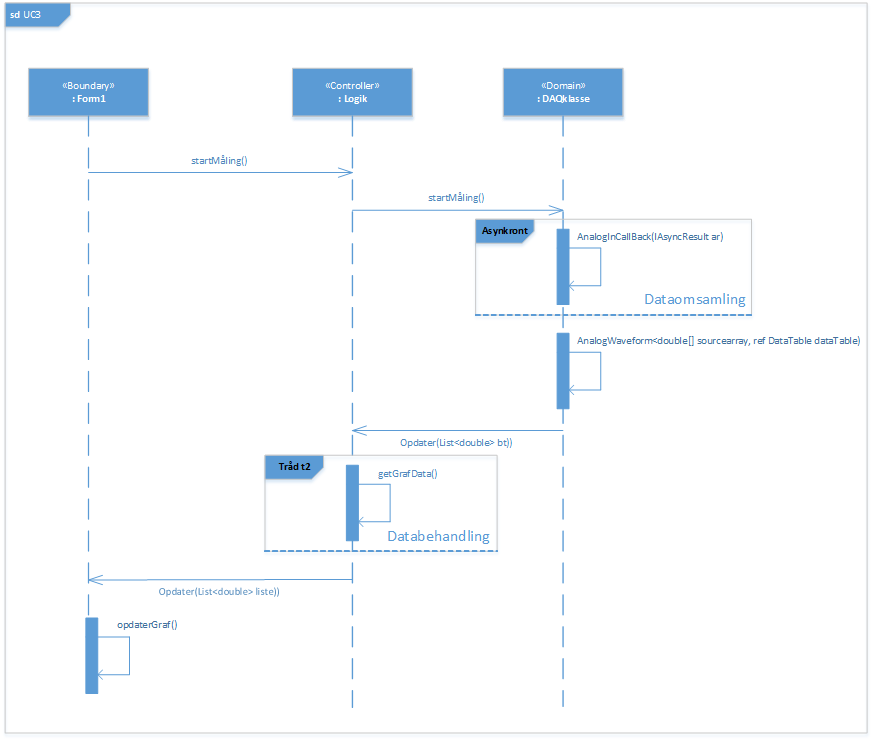
\includegraphics[width=1\textwidth]{Figurer/Softwareimplementering/UC3_sekvens}
	\caption{Sekvensdiagram for UC3}
	\label{UC3sekvens}
\end{figure}

Sammenspillet mellem klasserne i hele systemet er beskrevet i klassediagrammet på figur \ref{komposition}. For overskuelighedens skyld er metoder og attributter udeladt, og disse kan ses i dokumentationen afsnit 4.2.4:
\begin{figure}[H]
	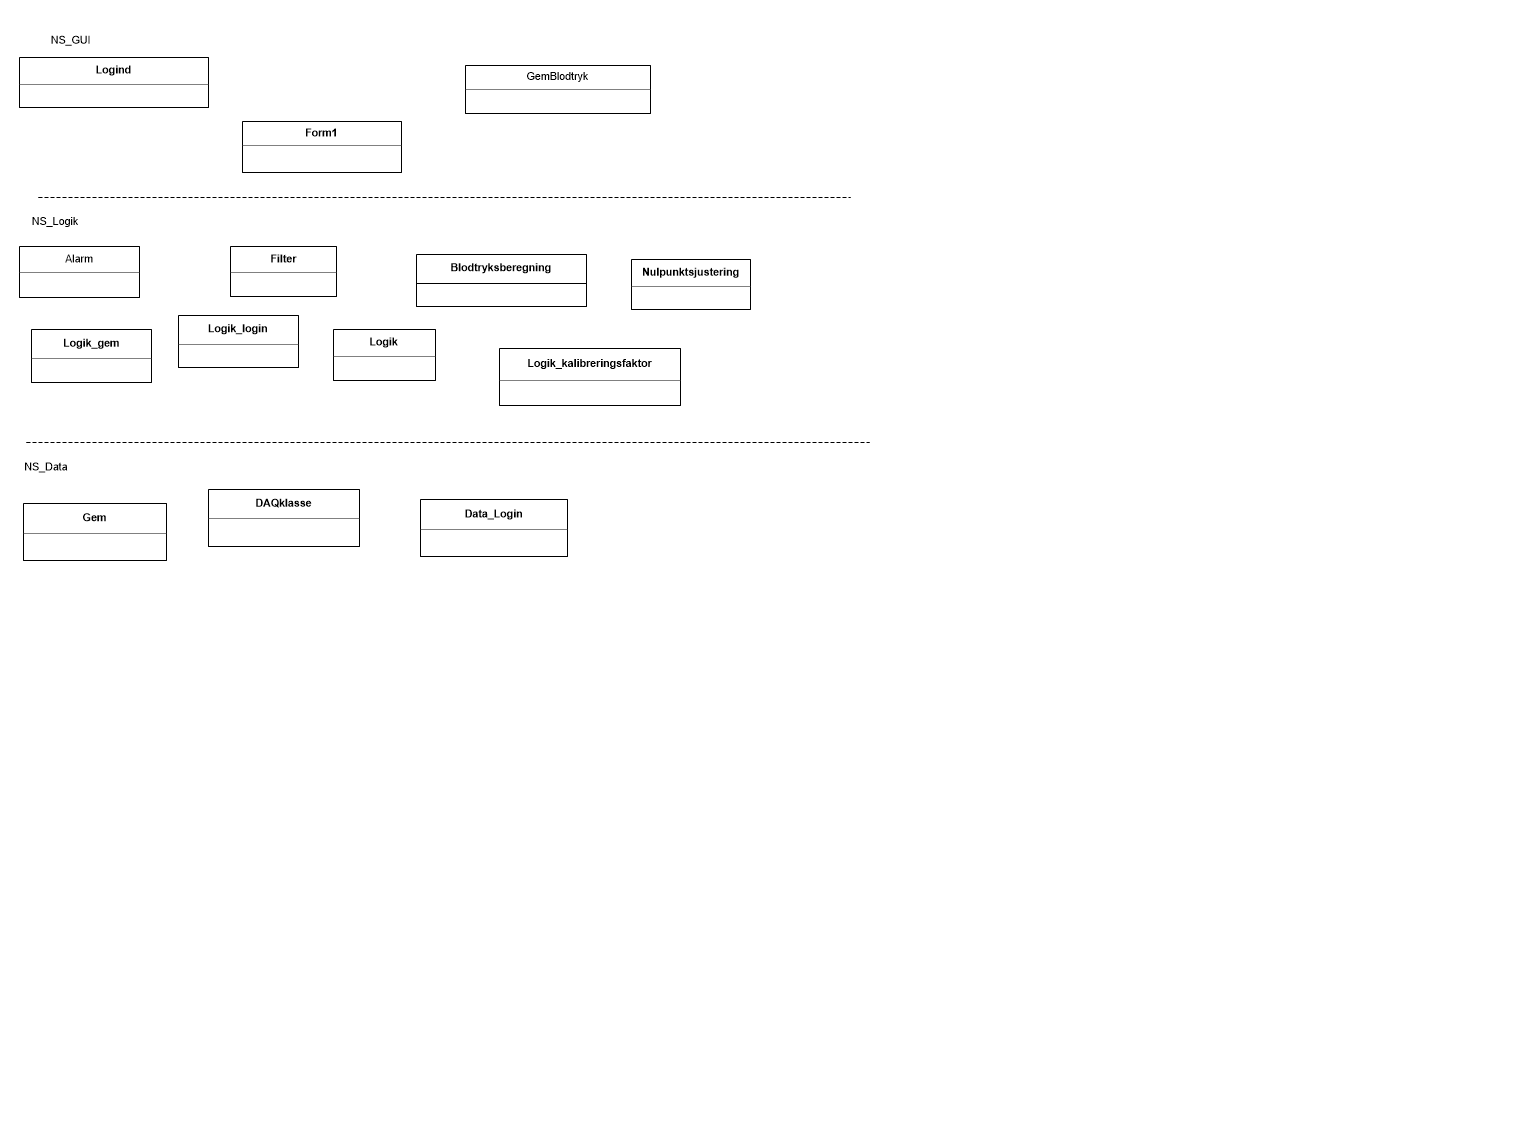
\includegraphics[width=1\textwidth]{Figurer/Softwareimplementering/komposition}
	\caption{Forholdet mellem software-klasser}
	\label{komposition}
\end{figure}
Ud fra figur \ref{komposition} ses det, at nogle af klasserne har komposition imellem sig og andre har en association. Kompositionen mellem to klasser fortæller, at den ene klasse opretter den anden, på samme tid, som den selv oprettes. Association fortæller, at klasserne har kendskab til hinanden, men de starter ikke samtidig. 


\section{Test}
Der er løbende blevet lavet tests på systemet i form af  modultests, integrationstests og slutteligt en accepttest, som blev udført under observation af vejleder.\\ 
I de indledende modultest af hardware blev det eftervist, at forstærkeren har en forstærkning på tilnærmelsesvis 400 gange. Ligeledes opfyldte det analoge filter tilnærmelsesvis kravet om, at have en knækfrekvens på 50Hz, idet modultesten af filteret viste, at den reelle knækfrekvens ligger lidt over 50Hz. Ved de senere integrationstests af hardwaren blev det eftervist, at forstærkeren og det analoge filter virker efter hensigten når disse er koblet sammen. I den sidste integrationstest af hardwaren blev det vist, at systemet med stor nøjagtighed i forhold til teorien kan levere et spændingsoutput svarende til det trykinput som transduceren leverer.\\[2ex]
Modultesten af softwaren har vist, hvordan de enkelte dele, i form af metoder og klasser, fungerer efter hensigten. Testen har vist, at der er overenstemmelse mellem det forventede resultat og det faktiske resultat, ved test med et kendt signal. \\
Integrationstesten af softwaren viste, at der var overenstemmelse mellem det indsendte signal og den graf og de værdier, der blev indlæst og vist i programmet.\\[1ex]
Ved integrationstesten af systemet kunne det ses, at værdierne, der blev opfanget i programmet, passede nogenlunde overens med de værdier, som kunne ses vha. oscilloskopet i Analog Discovery. Dette gjaldt både værdierne for det atmosfæriske tryk og trykket i væskesøjlen. Desuden kunne det ses, at programmet viste et blodtryk i mmHg, som tilnærmelsesvist var lig det teoretiske tryk udregnet for væskesøjlen. \\[2ex]
Ved accepttesten blev samtlige krav fra kravspecifikationen testet. Analog Discovery's signalgenerator blev sluttet til forstærkeren, som var forbundet til det analoge filter. Fra det analoge filters udgang var der forbindelse til DAQ'en, som havde forbindelse til en computer, hvor programmet var kørende.\\
Fra Analog Discovery blev systemet påtrykt et blodtrykssignal. På baggrund af denne opstilling blev use case 4, 5 og 6 testet og godkendt.\\
Til test af use case 1, 2 og 3 blev Analog Discovery udelukkende brugt som spændingskilde. En vandsøjle med kendt tryk blev koblet til en transducer, der blev koblet til systemet. Disse tre use cases blev ligeledes gennemført og godkendt. For dybere beskrivelse af test se testafsnittet (kapitel 5) og accepttest (kapitel 6) i dokumentationen.

\section{Resultater og diskussion}
Hovedkravene til dette projekt var at udarbejde et elektronisk kredsløb med indbygget analog filter og en forstærker, der forstærker signalet fra en transducer. Yderligere var der krav om at udforme en software, som kunne afbillede signalet fra hardwaren grafisk og som funktion af tiden. Desuden var der yderligere en række krav til softwaren, specificeret i afsnit \ref{Krav}. Det lykkedes at udarbejde et produkt, som opfylder alle disse krav. \\[1ex]
For at sikre systemet imod uvedkommende skal man igennem et login-system, hvorefter det er muligt at starte en blodtryksmåling. Der kunne med fordel være implementeret en funktion, som gav mulighed for at igangsætte en blodtryksmåling uden om login i tilfælde af en akut sag.\\ Et lignende login-system ville også være passende før kalibrering kunne foretages.\\
Selve blodtrykssignalet vises i blodtryksvinduet som funktion af tiden, dog uden aksebenævnelser på grafen, som vist på figur \ref{blodtryk}:

\begin{figure}[H]
	\centering
	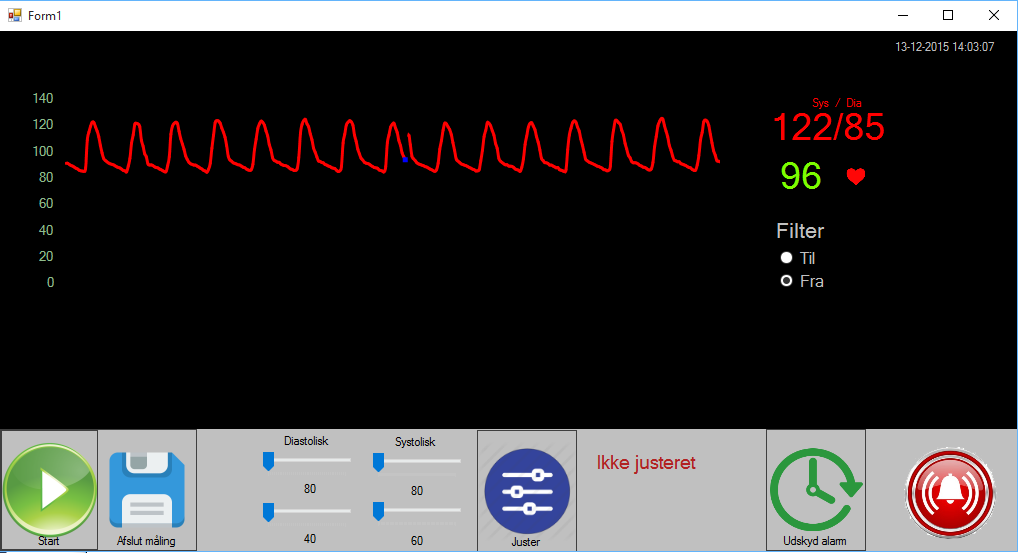
\includegraphics[width=1\textwidth]{Figurer/SoftwareImplementering/blodtryk}
	\caption{Blodtryskmåling}
	\label{blodtryk}
\end{figure}

På figur \ref{blodtryk} ses det, at det er lykkedes implementere funktioner, som digitalt filter, alarmering og visning af systole, diastole og puls. Dog opstod der problemer med at få den faktiske tid, det tager at nå hele aksen igennem, til at stemme overens med den beregnede tid.\\
Efter foretaget måling er det muligt at gemme data med tilhørende informationer i en lokal database, hvilket er afbildet på figur \ref{databasegem}:

\begin{figure}[H]
	\centering
	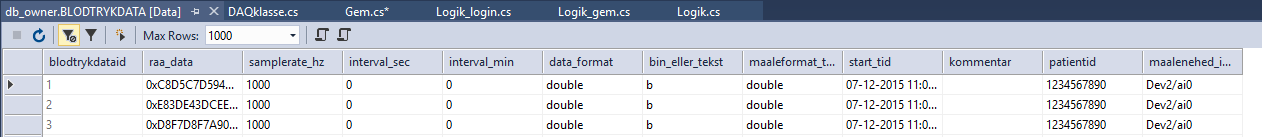
\includegraphics[width=1.1\textwidth]{Figurer/SoftwareImplementering/databasegem}
	\caption{Målinger i databasen}
	\label{databasegem}
\end{figure}

Signalet fra transduceren bliver igennem hardwaren henholdsvis forstærket og filtreret. Det har været et krav til forstærkeren, at den skulle kunne forstærke 400 gange. Igennem test kan det ses, at der tilnærmelsesvis opnås en forstærkning på 400 med forbehold for måleusikkerheder. Et problem har været, at Analog Discovery’s målescopes på indgangene ikke har kunnet opfange den størrelse signaler, der arbejdes med, grundet Analog Discovery’s offset. Når der tages højde for offset, nærmede den målte forstærkning sig 400. \\
Et krav til det analoge filter var, at den skal have en knækfrekvens på 50Hz. Ved modultesten kunne det ses, at knækfrekvensen minimalt oversteg de 50Hz, hvilket skyldes, at der ikke arbejdes med ideelle komponenter. Dog stemte den målte amplitudekarakteristik tilnærmelsesvis overens med den teoretiske. \\
Da forsyningsspændingen var +/- 5V, kunne forstærkerens udgangssignal ikke være højere end ca. 4,2V og filterets udgangssignal kunne ikke være højere end ca. 3V. Dette medførte, at signalet endte med en spænding på +/- 3V. Herefter, for at kunne udnytte DAQ’ens dynamikområde bedst, blev signalet sat maksimalt +/- 2,5V, svarende til en indgang på DAQ’en. Ved valg af en større forsyningsspænding ville signalet være blevet forstærket yderligere således, at signalet kunne sendes ind på en af de højere indgange med +/- 5V. Dette kunne føre til en bedre udnyttelse af DAQ'ens dynamikområde.\\[1ex]
Senere i forløbet blev det samlede system testet i CAVE-lab, hvor der var mulighed for at simulere et fysisk blodtrykssignal. CAVE-labs blodtrykssimulatorsystem var koblet til et blodtryksmålingssystem fra Siemens, som til dagligt bliver brugt på hospitaler, samtidigt var blodtrykssimulatoren også tilkoblet vores eget blodtryksmålingssystem. Ved målingerne var de udskrevne værdier og grafer for begge systemer mere eller mindre identiske, hvilket flot illustrerer, at projektet er kommet i mål med at udvikle et fuld funktionelt og nøjagtigt invasivt blodtryksmålingssystem. 
\\
Yderligere forbedringer til systemet kan læses i afsnit \ref{fremtid}.\\



\section{Opnåede erfaringer}
I løbet af projektet er der generelt opnåede erfaringer om, hvordan man indgår i et professionelt projektsamarbejde med projektstyring. Vi har især opnåede værdifulde erfaringer omkring, hvad man gør, når man har to grupper, som arbejder på forskellige produkter, der til sidst skal fungere samlet. I projektet blev der arbejdet med en software-del og en hardware-del.  Vi erfarede, at vi havde forskellige forventninger til, hvad der reelt skulle ske, når et software-system, skal arbejde sammen med et hardware-system. \\[2ex]
Projektet har givet indsigt i arkitektur- og udviklingsfasen omkring hardware. Hardware-udviklingen har desuden givet forståelse for eventuelle problemer, der kan opstå, når der arbejdes med reelle komponenter. Vi fik mange erfaringer med elektrisk måleudstyr, især når der blev arbejdet med små spændinger. Dette er meget relevant for os, som sundhedteknologer, hvor man arbejder med tilsvarende spændinger i sundhedssektoren. Vi fik meget hands-on erfaring med kalibrering, hvor vi indtil videre kun har arbejdet med teorien omkring det. \\[2ex]
Projektet har desuden givet os yderligere indblik i udvikling af et software-system, som skal arbejde sammen med en database. I softwaren er der blevet arbejdet meget med det nye begreb mønstre, specifikt observer-mønstret. Vi har desuden fået praktisk erfaring med programmeringsbegrebet tråde og tråd-synkronisering, idet vores software arbejder med samtidige processer. Vi har desuden arbejdet meget med digital signalanalyse, når vi har håndteret blodtrykssignalet, i vores program. \\[2ex]
Endeligt har vi udvidet vores fysiologiske viden, da vi i dette projekt har arbejdet med blodtryk. Vi har udforsket teorien bag  blodtryk og har i denne sammenhæng arbejdet med hæmodynamik for at kunne forstå præcise sammenhænge imellem resultater og målinger. \\

\section{Fremtidigt arbejde} \label{fremtid}
Gennem projektet er der arbejdet med det analoge filter og forstærkeren på to forskellige fumlebræt, fremadrettet kan man slå filter og forstærker sammen på et print. På den måde kan man undgå løse forbindelser som der let kan opstå i et fumlebræt.\\[2ex]
På længere sigt vil man med fordel kunne sætte DAQ’en, analogt filter, forstærker, strømforsyning og skærm sammen i en boks, hvortil transduceren er tilsluttet. Ved at inkorporere undgås for mange løse delkomponenter af systemet på operationsstuen, hvorved rengøring af udstyret lettes og i øvrigt fremstår mindre kompliceret over for personer uden dybere tekniske kendskab til systemet. Ulempen ved denne løsning kan dog være, at systemet er noget sværere at vedligeholde, idet hver enkel hardware-blok er afhængig af hinanden for, at systemet er funktionelt. Ved en eventuel fejl i en af de underordnede blokke vil det altså være sværere at udskifte en enkelt blok, eller det kan måske ligefrem økonomisk bedre betale sig at skifte hele boksen, hvorved der opstår et stort elektronikspild.\\[2ex]
Fremadrettet skal systemet udvikles med to skærme og kobles op til EPJ. Således at EPJ for den patient, der bliver målt på, kan stå åben på en skærm samtidig med, at målingerne foretages og vises på den anden skærm. På den måde vil den sundhedsfaglige kunne se informationer om patientens medicin, tidligere blodtryksmålinger og andre relevante informationer, der kan være vigtige for blodtryksmålinger på patienter under en operation. Desuden er det en mulighed, at de målte data efterfølgende kan gemmes i EPJ.\\[1ex]
Som systemet er nu, skal kalibreringsfaktoren udregnes manuelt. En fremtidig løsning hertil, kunne være at kalibreringen foregår i softwaren således, at man indsætter de tre trykværdier, hvorefter systemet selv foretager den lineære regression og udregner kalibreringsfaktoren. \\ [1ex]
Når der i den nuværende software for systemet indsendes et signal, der burde have en varighed af 10 sekunder, tager det programmet 16 sekunder at løbe igennem signalet. I fremtiden er det selvfølgelig meningen at denne tidsforskel mellem input signal og det viste signal skal elimineres. Således at disse to stemmer overens.\\[1ex]
For fremtiden er det meningen at systemet skal afspille en "bip"\--lyd for hvert pulsslag som systemet måler på patienten. I forbindelse med dette kunne alarmen også videreudvikles til at afspille højere pulslyde ved eksempelvis stigende puls. \\[1ex]
Selve brugergrænsefladen kunne udvides, således at blodtryksmålingssystemet bliver mere omfangende, med eksempelvis visning af et EKG-signal samtidigt.\\

